% !TeX spellcheck = en_US
\documentclass[11pt,a4paper,twocolumn]{book}
\usepackage[latin1]{inputenc}
\usepackage{amsmath}
\usepackage{amsfonts}
\usepackage{amssymb}
\usepackage{graphicx}
\usepackage[table]{xcolor}
\usepackage{wrapfig}
\usepackage{multicol}
\usepackage{multirow}
\usepackage{paralist}
\usepackage{longtable}
\usepackage{tabu}
\usepackage{soul}
\usepackage{titling}
\usepackage{pdfpages}
\usepackage[hidelinks]{hyperref}

\hypersetup{
	colorlinks,
	citecolor=black,
	filecolor=black,
	linkcolor=black,
	urlcolor=black
}

\title{Overmare's Journal}
\date{\today} 


\begin{document}
	
	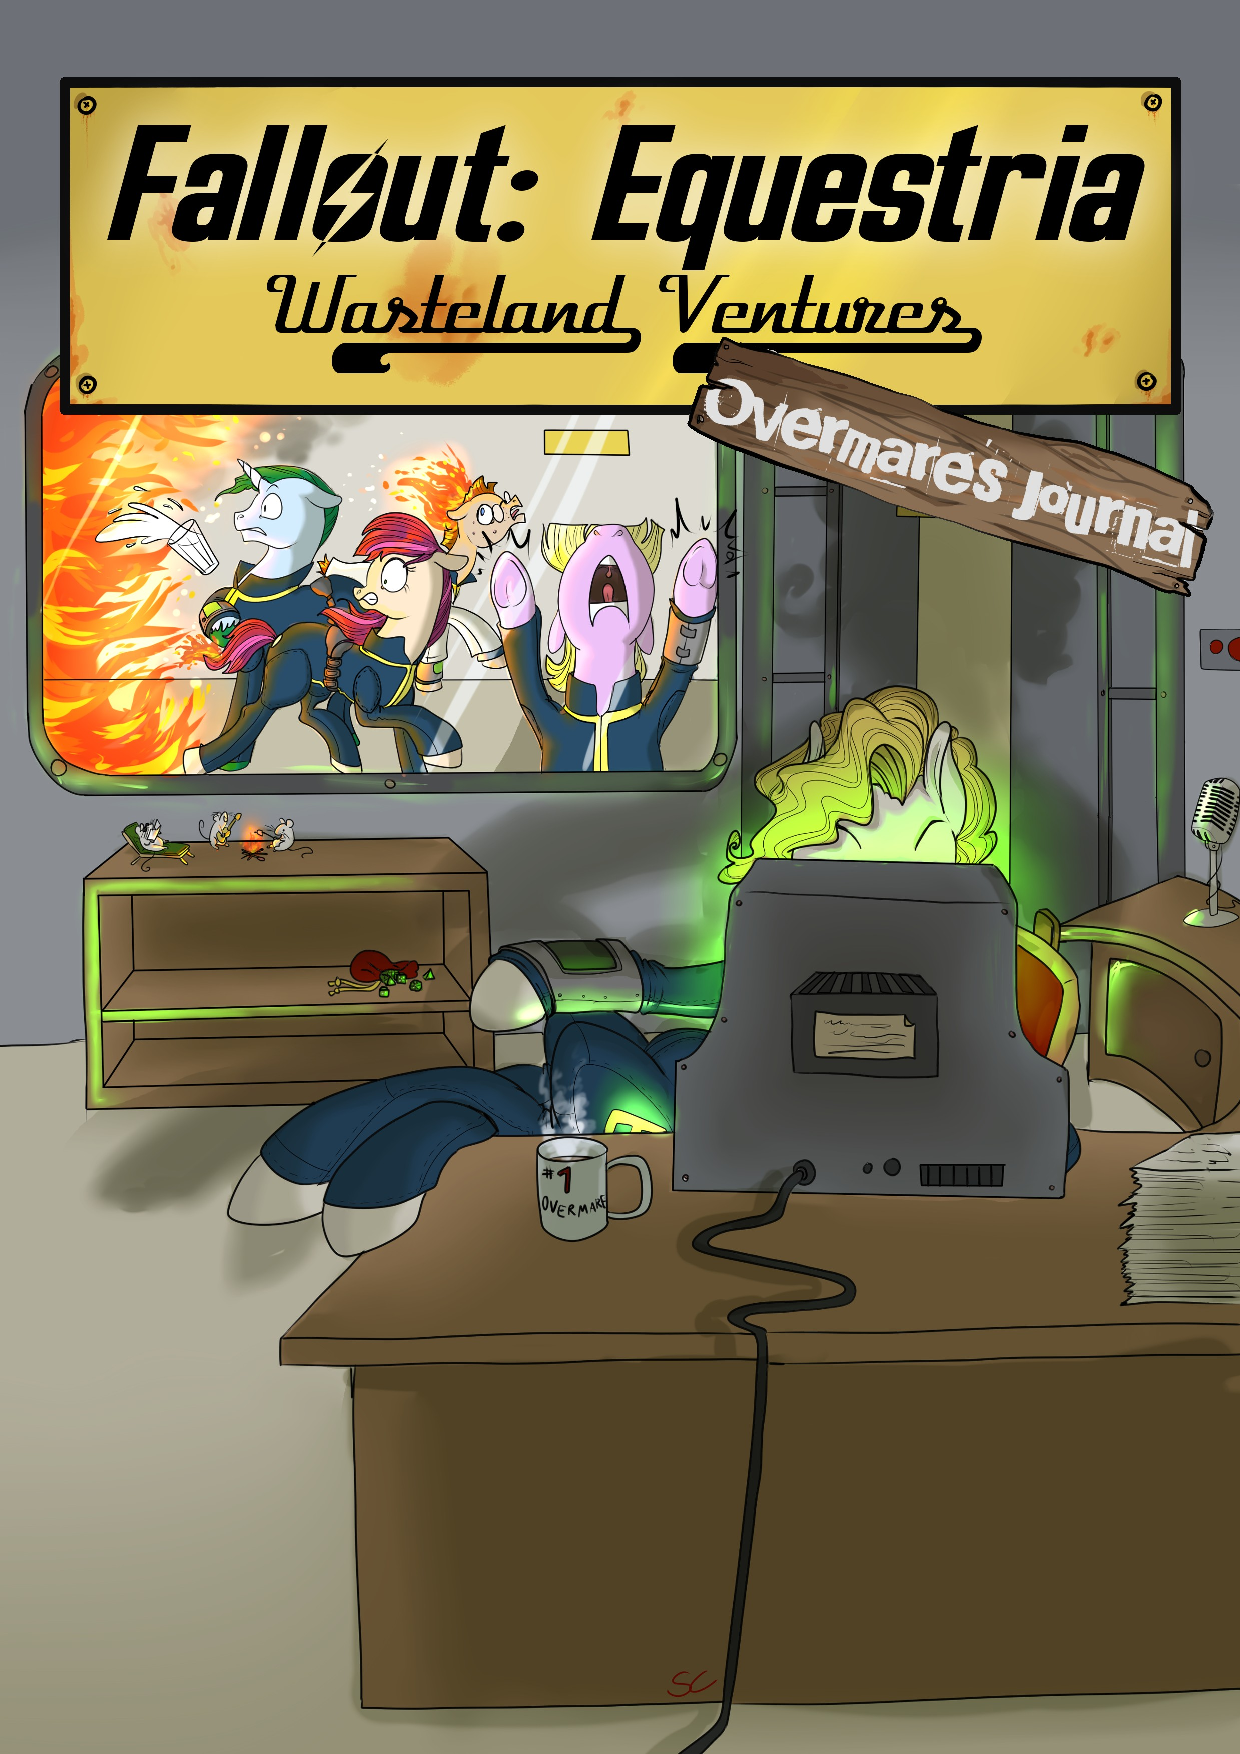
\includepdf[pages={1}]{WORD/COVER-OVERMARE.pdf}	
	\onecolumn	
	\setcounter{page}{1}
	\begin{center}
		Compiled by Waak, Kireanikin, LaPa, Miksu \& SourCherry
		
		\bigskip
		\textbf{Cover and Graphics:} SourCherry
		
		\bigskip
		\textbf{Layout:} Waak

	\end{center}
	
	\vfill
	
	\begin{center}
		\textbf{Version 2.3.0}
		
		\emph{Last compiled on \thedate}
        
        \emph{\textbf{Contact:} wasteland-ventures@googlegroups.com}
	\end{center}	

	\begin{figure*}[bp]
		\centering
		\includegraphics[width=3cm]{Art/ISA_Logo}
		\label{fig:isalogo}
	\end{figure*}

	\twocolumn
	\tableofcontents
	\chapter{Introduction}
    
    \begin{quote}
    \emph{The Overmare's Journal is a Stable-Tec Standard Guide Document for any new aspiring Overmares to embrace their roles as supreme leaders of each Stable. As such, it is vital no unauthorized eyes are to see this document for the safety and stability of the Stable.}
    
    \emph{- Apple Bloom, President of Stable-Tec}
    \end{quote}
     
    The Overmare's Journal is the Game Master's Guide to handling the interaction between the characters and the Equestrian Wasteland. The \textbf{Fallout Equestria: Wasteland Ventures} Core Rulebook has the necessary info players need to know how to play. This book contains additional information to help a GM - both old and new - to create and run exciting campaigns.
    
    For the sake of simplicity, this manual mainly focuses on group games, with more than one player beside the GM.
    
    Most of the information that should not be seen by players' eyes is located in this document, as well as helpful tips for GM-ing and other things to ease a new GM into their role.
    
    \chapter{Of Players and Game Masters}
    
     \begin{quote}
    \emph{Okay, grab your pencils, sheets, snacks and dice and let's get this game started! ...Where did I put my notes?}
    
    \emph{-Gaffer, the local GM of Ogres and Oubliettes from Junction Town}
    \end{quote}
    
    \section*{Rules of the GM-ing}
    The undeniable, all else overriding rule of any game for any GM, is to remember that the game is and will always be for the players. Players seek entertainment from the game, and game must provide such for the players to return for the next session. GM should be lenient and adaptive, capable of overlooking or altering rules for the group benefit. GM must show initiative for unpredictable events players might bring forth, respect the shortcomings of their actions, be able to reward ingenious or insane plans and their successes, and present politely the aftereffects of players' actions, and their impact to the game.
    
    The second most important rule is, that as long as there are more than one player, it is a group game, and every participant has an equal voice. At any given time it is not alright for one player to dictate the group's actions. It is GM's duty to uphold this and give equal attention to everyone within the session, even during times of dialog between the GM and a single player.
    
    Third rule is GM always has the final say on the matter, thus any conflict between characters, players and GM should always be ended by the GM as soon as it starts. Matters concerning rules and playing are fine to be discussed before the session, during breaks and after the session.
    
    \section*{Different players}
    Both new and experienced players might take part in the game. Their knowledge on the ruleset will vary, and it is vital to teach rules to new players and correct mistakes.
    
    As every player will be different, their contribution to the game will differ. Some might be quiet and take their time to proceed with their turn, while others can be highly active and talkative, often even trying to act on someone else's turn. Although it might be rude to rush someone to act faster, it is, however, greatly suggested to silence those who try to hurry themselves past others turns.
    
    Players can have very different personalities in and outside of game. Certain themes and subjects might go against either their own personalities, or just their character. It is important to know things characters do, does not always reflect to their players personalities. The game is always a fantasy, and players can be whatever maniacal genocidists, purest saints, simple minded fools, and anything they desire. Only limiter will be the game, giving the characters a certain mindset to begin with, be it criminals, neutral, or saviours.
    
    Fights between characters are part of normal gameplay and different opinions. While such situations are not praised, accepting them and keeping their tone calm is important.
    
    Fights between players are not acceptable at any time. Constructive discussion on someone's play is allowed, but it must follow polite etiquette. Rule of fun is always in effect.
    
    \section*{Character creation}
    As characters will be part of a story, and they may represent certain factions, it is important to give players clear idea, what their characters' public personalities should be like. While it is okay to have personal quirks that that do not occur in public, making open sadists representing law and justice, is an absolute no. Law and order however, can be achieved by such means.  
    
    Since the game is a group game, and as such it is suggested that players divide their roles, so that each player would be good at something, mediocre at elsewhere and bad with the rest of the talents. Examples are a speaker, a healer and a technician.
    
    Depending on the story, and the setting told, it is wise to give players a sense what kind of Skills characters would need. Any game that features combat, may leave characters without said Skills helpless, and thus affect the enjoyment of the controlling player.
    
    Characters' backgrounds are P.A.S.T. While mechanically, all they dictate is what skills the character has had experience in, to a GM they can be a potential treasure grove of material. Likewise, the character's actual past is one that a GM should utilize for maximum immersion of the players in the world. It is always a hoot having a character from your past suddenly approach you all of the sudden. Also, GMs can prod the players a little for extra detail in case they need it, without being too visible in their intent of having the character's past coming to haunt them.
    
    \section*{Railroading and open approach}
    The term \textbf{railroading} is used when players have little freedom to do what they want, and are instead forced to advance the story and abandon the exploration by the GM. As a roleplaying game, having excessive railroading is often frowned upon. It greatly limits player involvement, choices and approaches to everything the game dishes out. However, some amount of railroading is necessary, to keep story cohesion intact. However, it should never come at the expense of player agency. Nothing is more boring than making your players a spectator in their own story.
    
    Following cases allow railroading as a necessity:
    \begin{description}
        \item[One-shots:] One-shot games are single session games, often designed for ready made characters without character advancement. As such, they are within a limited play-area, with limited goals and options to complete. Thus, it is fine to enforce the story and events within to advance.
        \item[Time limit:] In situations where characters have to complete or prevent certain events within a time limit, for instance to stop a reactor from exploding, it is fine to give players incentive to move forward instead of wander around without rush. However, giving time limited events often is far too much railroading, and thus breaks the exception. 
        \item[Storymode] The game has been pre-informed as a story driven game, thus all players are aware of the railroad experience, and the limited nature of randomness and choices.
    \end{description}
    
    \textbf{Open approach} is the way of giving players a choice to move where they want, when they want. It allows players to abandon missions, return to them later, and even do completely opposite than the GM has planned for them to do; Enemies can become friends, innocent can be sacrificed, and the story can rewrite itself. 
    
    For a GM, this can be difficult to control and it can spiral out of control easily. It should be noted that when making an "Open World" so to speak, GM should be prepared to at least have important locations be such that they can appear almost anywhere in a map. Possibly with a new name, and the players ought to be none the wiser. This way, the story remains mostly intact.
    
    \section*{Dishing out death and resigning players}
    As players face the dangers of the Equestrian Wasteland, whether it is the people, or the remains of the Great War, death is ever present. At some point, players may make mistakes, face odds they can't win, or simply roll terribly, the death might come to the character. It becomes the GM's duty to decide whether they wish to kill a character, or simply injure them seriously. For the enjoyment of the players, it is wise to avoid killing characters needlessly. However, suicidal behaviour, such as an extreme example, facing against an army with a BB gun should be punished with death. On the other hand, a comical approach would also have the army simply punish the character with other methods than death.
    
    As campaigns are often long running, it is possible for a person to be unable to continue the game within the time schedule the game is being played, or having grown tired of the game. Thus, the character is often played out of the game. The most memorable way to do this is killing the character off. It affects the rest of the group, and shows them their mortality. In addition to this, it is often a good roleplaying moment, even if the event itself is undesirable. Be willing to apply a Rule of Cool in these situations.
    
    Killing or just injuring the character out of commission should be swift, unexpected and shocking, stunning the other characters. This make them unable to save their comrade, rather than letting the situation drag on and on, thus lessening the impact of what should be a shocking moment for the characters.
    
     \section*{Campaigns and one-shots}
    Campaign is a collection of sessions, normally with same characters that advance as the story progresses and experience is gained through actions and hardships of the characters journey. Campaigns have a story that can be either very loosely followed as a main goal to be achieved whenever, or have a sole purpose that ties everything within the game together.
    
    One-shot games are single session games, often designed for ready made characters without character advancement. As such, one-shot games are often a good way to teach new people the basic rules and how the game is played. As players rarely have time to get attached to these short living characters, dishing out death to them is much more easier and acceptable. 
    
    There is usually a single goal the players are supposed  to complete. Thus, it is fine to limit players, where they can go, and what they can do, since their participation is only for this session. However, one-shot games can be part of a campaign. They can be the prologue to set the tone and lore, an epilogue to wrap the campaign up, or an event that takes part within the time span of the campaign.
    
    \chapter{War Never Changes - Lore}
    
    \begin{quote}
    \emph{"Once upon a time, in the magical land of Equestria, there were two regal sisters who ruled together and created harmony for all of the land..."}
    
    \emph{-Twilight Sparkle, Ministry Mare.}
    
    \end{quote}
    
    This first chapter of the Overmare's journal is dedicated to the setting and tone of your games; post-apocalyptic world with pastel-colored equines. It is recommended that Game Masters new to the setting read the source material, Fallout: Equestria by Kkat, but we do our very best to bring you the gist of it in this chapter. 
    
    \section*{Ministries}
    
    \textbf{Ministry of Arcane Sciences} (MAS) was dedicated to the study and development of modern magic under supervision from Twilight Sparkle. Her Ministry would create many of the most potent horrors a Wastelander knows, most notable being Impelled Metamorphosis Potion (I.M.P.), colloquially known as "Taint". This creation subsequently caused the creation of many mutated horrors after the war, including Hellhounds and various abominations. Their most significant research was to the creation of artificial Alicorns which succeeded and went horribly wrong at the same time.
    
    \bigskip
    
    \textbf{Ministry of Image} (MoI) was responsible for graphics and imagery for the wartime effort, quickly becoming a propaganda-machine with its altered or outright banned book lists and destroying of unpatriotic books. This ministry largely went unnoticed by the populace, yet its supervisor, Rarity had her hooves deep in dark magic, all with good reasons, of course. Much of the posters that have remained plastered to walls in the Wasteland buildings were produced by MI.
    
    \bigskip
    
    \textbf{Ministry of Morale} (MoM) begun and paraded as the ministry that would dedicate themselves to keeping the civilians happy and carefree of the war. Behind the public eye, however, this ministry was dedicated to rooting out traitors aiding the zebras. This was made possible by the invention of Spritebots and with memory spells. The ministry was directed by Pinkie Pie, and this ministry was the least subtle about its covert operations. 
    
    \bigskip
    
    \textbf{Ministry of Wartime Technology} (MWT) was dedicated to development and improvement of new weapons and armor largely meant to help the common soldier, with a smaller branch focusing on every-day items. Their most significant development was that of power armor; a suit of magical armor capable of withstanding heavy attacks and administer healing potions and spells should the need arise. 
    However, the leaders of the various companies that made up the board of this ministry were discovered to be corrupt by it's director, Applejack, which led into the Ministry's turmoil.
    
    \bigskip
    
    \textbf{Ministry of Peace} (MoP) was responsible for the research into medicine and healing spells, and many hospitals operated in this ministry's name. Though well-intended, this was the ministry that ultimately doomed the world by inventing the megaspells, originally intended as massive healing spells.
    
    \bigskip
    
    \textbf{Ministry of Awesome} (MoA) was the most subtle of the ministries, having seemingly no public purpose at all. However, this ministry directed by Rainbow Dash, was dedicated to many black ops operations behind the scenes and bleeding edge research.
    
    
    \section*{Regions}
    
    The Wasteland is vast and varied in environment, from frozen north to the thick, necrotic pinewoods of south and blazing hot deserts in the west. This part focuses on giving GM's at minimum the general sense of what the world is like and at maximum offer setting ideas with bustling, vibrant settlements for near-instant playability.
    
    This section focuses first on the Equestrian Wasteland and its regions divided into five areas: north, east, south, west and central Wasteland. After that, it is the same regions for Zebra Homelands and Griffon Territories.

    \bigskip
    
    \subsection*{Central Equestria:}
    
    Central Equestria is an area with a tempered, once lush and green terrain, now replaced with dead woods and dusty hills. The temperature is pleasant, which means that population has settled in, both ponies and mutants alike. The former crown jewel of Equestria, Canterlot, is a well-known landmark, visible even far away due to its mountainous location.
    
    \subsection*{Canterlot}
    \textbf{Location:} Central Equestria
    
    Canterlot ruins is the former capital of the pre-war Equestria, now illuminated by a lethal pink haze. Its only inhabitants are Canterlot ghouls, a particularly enduring and nigh-unkillable subtype of ghouls, as well as skeletons from a bygone age. The buildings are in a state of strange preservation, as the Pink Cloud has seeped into every stone, every bone and every dead tree. While some buildings have not withstood all 200 years intact, the buildings are overall in a better shape than most. That is, if the air wasn't poisonous and incredibly radioactive. Likewise, radio broadcasters in Canterlot emit a lethal static.
    
    However, the ruins are not entirely without civilization. Canterlot Ruins holds within it Necropolis, a settlement of ghouls that live underneath the ruins, and are for the most part peaceful and sane. However, they are perfectly content on spending their time away from Wasteland's ire.
    
    Inside Canterlot ruins are various government buildings, including Ministries' buildings and the Canterlot Castle, home of the two Royal Sisters. Canterlot also had Stable 1 as well, however the Stable's residents soon perished of the Pink Cloud seeping in.
    
    \subsection*{Everfree Forest}
    \textbf{Location:} Central Equestria
    
    \subsection*{Ponyville/Pon Evil}
    \textbf{Location:} Central Equestria
    
    Ponyville, or "Pon Evil" among the wasteland populace, is one of the oldest raider settlements in the wasteland. Perhaps due to the war-mongering nature of raiders, it has never been kept by one particular group for very long. Ponyville is also the origin of Stable 2, a stable designed to stay closed indefinitely, hidden within the premises of Sweet Apple Acres.
    The once beautiful pre-war town is now a mere shadow of itself, with destroyed, defaced buildings and grim reminders of its inhabitants' impulsive, volatile behavior littering the place. The air in Pon Evil is stagnant, and pungent with the smell of rot, gunpowder, and thick smoke from bonfires. The dirt roads are caked in blood of past firefights. 
    
    Notorious sights in the town are the remains of Golden Oaks library and the Government Hall, both packed to the brim with Raiders. It is worth mentioning that only a particularly foolish pony would venture into Pon Evil willy-nilly. The lethal, but botanically important Everfree forest is also at the edge of Pon Evil, a wild, untamed forest full of monsters and death. Even the raiders are not mad enough to approach it without a valid reason.
    
    \subsection*{Zebratown}
    \textbf{Location:} Central Equestria
    
    Located at the base of Canterlot mountain, Zebratown housed many, if not most zebra living inside Equestrian borders during the war. After rainwater and other sources of tainted water supply submerged the town in pink-hued flood, the town was quickly decimated. What is left of the town is a 200 year old ruin: it is also one of the few places where Canterlot Ghouls are a fairly common sight.
    
    \subsection*{South Equestria:}
    
    \subsection*{Appleloosa}
    \textbf{Location:} South Equestria
    
    A pre-war settlement that after the Great War ended, slowly became a slaver stronghold. Those that managed to flee with their lives rebuilt their home a solid distance away and named it New Appleloosa. The two are still connected by a track of railroad splitting the San Palomino desert.  
 
   
    
    \chapter{World of wonders and wrongs}
    
    The world outside, the wondrous Equestrian Wasteland is full of both excitement and despair. This chapter focuses on creating a compelling world for players to explore the unknown and forgotten, to enjoy the broken society being rebuilt through hardships, and to feel both triumph and defeat against odds.
    
    \begin{quote}
        \emph{\textbf{Example one-shot scenario:} A group of soldiers arrives to an unknown island, and are to scout the nearby ruins, and set up a base camp there. When the main story starts, those ruins have bunch of soldiers already settled in, and players are going to explore rest of the island.}
    \end{quote}
   
    \section*{Writing a story}
    
    Imagination. That would be the first word to begin writing a story with. It both starts and ends everything, it will not have any limit to it. And it is how this manual approaches story writing. 
    
    Creating a story does not have a clear guide to it, nor it should. Your imagination is your strongest asset, and helping it with any references from literature, games, movies, series and more is not only suggested but often mandatory for new writers. Through experience stories evolve. They are not always something that hook their players, keeping them entertained and on the edges of their seats. And that should never be discouraging.
    
    \section*{Creating a world}
    
    To start, using an actual location from any source material is a good basis for the creation of the game world. Towns, cities and other landmarks are easy to situate to a ready template with personal liking. An artistic person can draw their own map, and situate their locations how they desire.
    
    Next, the world needs details such as vegetation and plant variation, a possible season of year the game is being played in, and mountains and other hindering or isolating land formations to name few. These help to limit what kind of details players can expect from the world. For example, events of the game world can happen around one massive mountain that everyone tries to control. Questions come from what surrounds the mountain, and what makes it special for the story.
    
    Settlements of various sizes determine how civilization has recovered from the devastation of the Great War. They can be welcoming and humble, massive and corrupt, supremacists, near-hostile against outsiders, or even live in complete obliviousness of the outside world.
    
    Since the world is remains of a once strong civilization, landmarks, monuments of the old world fill the area. They may be equine and griffon made statues and structures. Remains of a now barren national park, lush swamps, caves and quarries.
    
    One important factor to bring out life into your game is varied NPCs, with their own problems and day-to-day life. Though it is not necessary to write a 10-page essay on every NPC you create -which you may end up having a lot of-, it is good to consider and have at least some kind of inkling of what kind of person the NPC is as a guideline to how they would act in situations. You can read more of this in Chapter 3: Encounters and interactions.
    
    \section*{What lurks among us}
    \textit{We are not born a monster, but become one through our actions. We do not choose to whom we are born, where we are born, nor when we are born. Only thing that matters, is how we proceed.}
    
    \bigskip
    
    The world of wonders is full of strange, unpredictable and questionable people. There are wealthy and thieves, victims and murderers, prey and predators, slaves and slavers, doctors and executioner, civilians and soldiers, and clients and providers. And all those, who stay within the gray area between, struggling to survive day after day with few caps and ends. 
    
    Easiest approach is to create societies with bad apples among the good and the humble. The world is likely to have poor and mistreated people, those who trample them, those who ignore them, and the few that assist them. The world is gritty, torn apart remnant of its former self before the devastation, and thus, those who seek commodities usually gain it through someone else's labour and pain.
    
    While creating an utopian world is compelling and sounds brilliant, it is often very difficult to make authentic. Thus, it is simpler to create certain locations within the world, that might have an isolated utopian society, that players can visit. As players interact with such societies, either party is bound to either change the other, or leave the other even more affirmed of their own visions. 
    
    \subsection*{Raiders:}
    An indefinable group of people, whose main lifestyle is raiding and ravaging through other settlements. Though often thought as little more than a drug addict with a penchant for unbelievable violence, it might be good to consider the reasons a character has fallen into this lifestyle. Were they born into it, or was it addiction or poverty that has driven them to extreme measures? Do they try to intimidate all others with over-the-top measures? Or perhaps they just have that liking for sadistic acts?
    
    Thinking about these reasons can make the NPC feel more alive and less like a prop or a tool of story-making. Still, a GM can try to balance the horrific acts with this background in mind, not needing to sacrifice the gritty for the sympathetic side. After all, most horrible people have their reasons to be so.
    
    \subsection*{Slavers:}
    An organized group, comparable to Raiders in their vile antics, Slavers make their living on both high priced loans and providing slaves. Those who cannot pay the loan back, are enslaved to work in imprisonment until someone pays off their debt, or buys them as slaves for their own personal use. However, it is not unheard of for Slavers to perform raids to settlements and travellers to acquire slaves by force. How the slavers operate is free for GM to change, so that they fit better to a setting.
    
    \subsection*{Steel Rangers:}
    The remnants of the Great War; originally the Power Armor they wear was meant to be a high-tech battle suit developed by Ministry of Wartime Technology, worn by soldiers in the front of the battle. Now those same Power Armors have became the trademark of Steel Rangers; tech-hoarding, isolationist ponies who think most Wastelanders are either too stupid, or careless to use said tech. 
    
    Bound by a strict Codex and even more hard-headed leaders, the group is not entirely just a bunch of crabapples; there are some ponies still guided by their good heart, that deflected this faction and formed a group of their own called Applejack's Rangers. Unlike the regular Steel Rangers faction, AJ's Rangers are focused on the betterment of Wasteland and Equestrian citizens, to honor the Ministry Mare who started it all with an idea of a Power Armor. These facts should be kept in mind when designing Steel Ranger or Applejack's Rangers NPC's. Think of their standing in the group, are they frustrated with it? Do they even think it is right? And if they do, why?
    
    \subsection*{Zebras:}
    The other side of the Great War, fighting against the nation of Equestria in a long, hopeless war. While we get no confirmation about the level of destruction of the Zebra Nation -that remains nameless to this day-, it can be reasoned that the destruction was two-sided. Today, most of the Zebra found in Equestria would technically come from two sources of ancestry: either they already were Equestrian citizens from well before the war and survived the apocalypse in Stable 3, or they were zebra operatives, spies and saboteurs who also managed to survive. 
    Most zebras now live in tribes, small communities that may or may not be away from pony populus, due to prejudice and old grudges that likely exist in both sides. Many zebra still hold onto their old beliefs and superstitions. When making a zebra character, it is good to keep in mind how they interacted with their tribe. Are they still part of it, or did they leave? Was it on good or bad terms?
    
    
    \subsection*{New Canterlot Republic:}
    A very new faction, formed during and after Littlepip's journey through the Equestrian Wasteland. They tend to take in nearly any who wish to join their ranks, though they might have some reservations or higher expectations towards characters with a known evil past, such as raiders, though they are more than welcome to join if they truly wish to redeem themselves. NCR can be thought to be the second-most bureaucratic faction, on par with Steel Rangers, so it is good to keep in mind that change -both good and bad- is slow to happen, and the faction can still have those with malicious intent or hunger for power in its ranks. 
    
    NCR is ruled by a President, who during and near the Day of Sunshine and Rainbows is \textbf{Gawdyna Grimfeathers}, a griffon of Talon Company fame.
    
    \subsection*{Local gangs, groups and thugs:}
    As settlements grow, so does the number of people inhabiting them. There has to be someone to keep order, and thus, groups of people usually gather under one or more leaders. They can be a settlement or area specific groups, both law abiding and criminal in nature. They can be the security of the settlement, work beside them or work against them. Their rule may be influencing from the background, or directly tyrannical. As these groups are limited in size, reputation outside and inside their controlled area is often unrelated.
    
    \subsection*{Alicorns:}
    Artificial beings created when a pony is dipped into Taint, a very powerful creature that is a feared sight by all Wastelanders. Though originally implanted with a hivemind and very specific skills, the alicorns would work together with NCR in the future, and have managed to get free from the hivemind.
    
    Before the rise of New Canterlot Republic, these mutants were led by Goddess, an alicorn created during the apocalypse, when some of the brightest minds in the Ministry of Arcane Sciences fell into the vat of I.M.P -Impelled Metamorphosis Potion-, now known with the monicker Taint. The Goddess is the one who commanded the other artificial alicorns in growing their ranks and perhaps managing to find a way to make male alicorns, as all ponies that were dipped into Taint, even if they were stallions, would turn into a mare upon emerging. That is to say that before Little-Pip's adventures, all alicorns are mares.
    
    At the same time, Alicorns can be both complex and simple for a GM to use as adversaries. Their goals are simple -get more ponies turned into Alicorns- but their hivemind, meaning no trick works on them twice, makes them difficult to manage in campaigns that do rely heavily on Alicorns. Alicorns, at least before the events of Fallout: Equestria, are difficult to make into nuanced characters, serving more of a always-evil antagonist. Though, this doesn't necessarily stop a GM from inventing work-arounds why a particular Alicorn character isn't properly linked to the Hivemind, allowing them to be more of a character in their own right, or other reasons why they stand out from the "herd".
    
    \subsection*{Grand Pegasus Enclave:}
    Grand Pegasus Enclave, or Enclave in short, is a civilization created by the pegasi that sealed the cloud cover at the end of the war. During the events in Fallout: Equestria, Enclave made their appearance with the clear intention of genocide of anything deemed impure or tainted with radiation. Much like other pony governments, the Enclave doesn't have a shortage of those with a hunger of power and control.
    
    Though much of the civilian and military life of the Enclave is shrouded in mystery, leaving ample grounds for Game Masters to create their own ideas of the civilization above clouds, some facts are known: the Enclave have been known to brand any who go against their ideals as Dashites, by burning a brand of a lightning cloud -Rainbow Dash's cutie mark- and exiling them to the Wastes below.
    
    They also have strict rules on family sizes, with higher ranking military officers given permit to have more children, while others are forced to one-foal policy in the name of making sure the population doesn't grow too large. In strict contrast to some settlements in the Wastes, homosexuality is encourages in the Grand Pegasus Enclave as a measure of population control.
    
    To a GM, the Grand Pegasus Enclave can strike that balance of having just enough info about them to give the basic gist of what the group generally is like, while still leaving enough room for personal ideas. It is welcome for a GM intending to use this group to think about how the culture might differ from town to town or how rigid they want to portray the members of this group, especially when serving as antagonists. Due to being ponies, they can be swayed, shown that not all Wastelanders are horrible people, or perhaps they're so rigid in their indoctrination that the fact doesn't matter to them?
 
    \section*{What lurks outside of us}
    The Equestrian Wasteland is inhabited by variety of mutants, animals and other creatures twisted and corrupted by Radiation or Taint. While some are intelligent, most are savage beasts; their motivation pure instinct of hunger, territory or offspring. Generally, such beasts cannot be reasoned with nor tamed, only distracted or scared with presence threatening enough. 
    
    Feral ghouls are ghouls whose long life and exposure to Radiation has broken their sentient brains, leaving them with only feral instincts. They often stay in crowds, clinging close to their old homes and familiar areas. Commonly, feral ghouls ignore sentient ghouls, unless agitated or assaulted.  
    
    The creatures are based on actual animals and mythical folklore beasts, thus their behaviour and occurrence depends on the time of the day, distance from the settlements and whether they are travelling in packs, duos, or alone. For instance, a pack of timberwolves, duo of radstags and a single radscorpion, are common sights.
    
    Beside animals, certain plants have transformed into life devouring monstrosities. 
    
    Among wildlife, there are robots, wonders of mechanics and arcane arts. These machines rely on code and procedures, that can be tampered with. Their configuration can be changed to ignore characters, turn against their previous owners or even shut down and forced to self destruct.
    
    All these creatures can be found in more detail in the \textbf{Mutant Manual}.
    
    
    
    \chapter{Encounters and interactions}
    \begin{quote}
    \emph{"Hey! You tell little miss Spring Roll to pay up her 100 caps, or she'll be losing more than just her home."}
    
    \emph{- Local thug in New Appleloosa.}
    \end{quote}
    
    As players travel the wondrous world, they ought to encounter various kind of characters of both good and bad intent. NPCs usually have some key-characteristics of some notion of personality, a name and body language. At the end of this chapter we include a small list of names to be used, but it is advised that each GM still think a name list of their own for the situations where -and these situations will crop up eventually- the players decide to talk to a random person to the left of your designated, well-thought-out NPC. 
    
    \section*{Creating encounters}
    Encounters are simplest way to effectively introduce NPCs, parts of the story, lore of the world, or just entertain players when story is being on hold. Encounters can be grouped to planned and random. 
    
    Planned encounters are usually part of the story being told, or side stories GM wants to hint for the players to fully participate. Their occurrence is usually tied to locations characters arrive, or triggered by actions they have made.
    
    Random encounters are events that either suggest a possible side story, or simply wish to give players something to do out of sudden. These events can occur at any time, often or rarely, even make repeating appearances. It is wise to create a variety of random encounters to be utilized whenever necessary.
    
    Building an encounter begins with an idea of what happens and where it takes place, as those can give insight what players will be up against. For example, Pre-War ruins tend to have different types of mutants mingling around than a swamp, and thus it is unlikely to find hydras hiding in the alleys.

%    Step 0:
%    Have an idea of the encounter, what happens in it and where it happens.
    The importance of the encounter matters. If it has an effect on the story being told, it will be better to present it in multiple occasions, with more or less emphasis. If it is simply an occurrence of daily lives in the Wasteland, it's presentation can be left to as minimal as possible.
%    Step 1:
%    Decide the encounters importance, is it part of the story or outside of it. 
%    This helps the next step. 
    How carefully and in detail the encounter is brought into players' attention, the more likely players can pick up on the importance of such encounter. However, a pushy presentation of an encounter can make it feel forced upon players, giving them less freedom to act during it. Or simply said, a railroaded event.
%    Step 2:
%    Design how the encounter is presented for the players. The more detail it has and the clearer it is being forced upon them, the more likely players are able to understand it's importance. However, too pushy presentation may leave the players feel railroaded, forced to go this one path instead of their own choices.
    
%    Step 3:
%    Design the encounter:
%    ●	What happens
%    ●	Where happens 
%    ●	When happens 
%    ●	Who are participating
%    ●	What happens if taken part of
%    ●	What happens if ignored
%    ●	Does it recur
%    ●	Difficulty to succeed
%    ●	Difficulty to fail
%    ●	Reward for success
%    ●	Penalty for failure
    
    When designing the encounter itself it is wise to make a few short key points to keep the important details in mind. Note that reaching the various stages of the encounter should be left to the players to handle. You can make a list of short key points: what starts the encounter, what time of day it is? Who are participating, and if they are new characters, what do they look like? What happens if the encounter is taken part of, what if the players decide not to partake, are there long-lasting effects if the event is ignored? How easy is the task at hand? What are their rewards for success? 
    
    Unfortunately, this doesn't necessarily prepare for all the possible outcomes the players can come up with:
%    Step 4:
%    Give the encounter a time schedule. This will make it simple to follow when the encounter should be given to the players and when they have to get parts of it done, or fail.
    you can come up numerous options and approaches to tackle your encounter, and your players can still come up with more and more ideas you will have to improvise on. Sometimes, these can be the kind of improvisations that you're thankful for. In situations like these rewarding the players for their ingenuity is the course of action: if their plan or solution is sound, work that solution in and let them continue on that path. At the same time, anything suicidal or stupid should first be double checked from the players, if they truly want to continue with it. If they do, play it out however fittingly you see it. 
%    Step 5:
%    Prepare for the unexpected and improvisation. Players might do things GM couldn't even imagine to occur.
    

    \section*{Handing out quests}
    Tasks, jobs, quests, work, missions, assignments, chores, errands... Different words, same meaning.
     
    The game most often begins with a sole quest the characters either begin with, or receive at the beginning. However, handing out side quests, random encounters and even parts of the main story can be tricky at times. Depending on the players, quests can be actively sought by the characters by interacting with NPCs and other sources, or only be presented by the GM.
    
    How quests are given depends greatly on the place they are given. A small camp of people can actively ask for help from the player's characters, where as a big town can give them after some interaction with the people.
    
    \textbf{Notice board approach:} When dealing with either a large society with numerous people giving out work, or being part of an organisation that receives requests, a notice board for quests is a possible choice. These notices can have small description telling what the task is about, who is giving it, where they are and what the reward is. 
    
    \section*{Designing NPCs and their behaviours}
    To make varied and interesting NPC's, it is important to set them apart from one-dimensional characters. This can be done by writing down some main facts about the NPC; their personality, maybe note how they react to certain kind of situations, such as utter strangers -which often end up being your players' characters the first time they meet said NPC- suddenly coming to talk to them. This list of traits can be just a list of musings and thoughts, but they do flesh out the character.
    
    After you have figured out your NPC's main personality, it is time to give them a distinct "voice". This doesn't necessarily have to be a mere vocal accent -though if you can, it is greatly encouraged to give feel to the character- but also the way the character moves, behaves and walks. For example, if the NPC is very shy and reclusive, the GM may bring this out in their own acting -if the players are around the same table- by hunching back slightly, speaking with a lower volume or by stuttering and avoiding eye-contact. 
 
    Or if the character is boisterous and brave hero of the Wasteland, act out their body language; lean forward, speak in higher, brazen volume and if you can, maybe even stand up. 
    
    If the character is angry, they might speak in hissing tones, and their body-language is shutting others out; ears go against their head, they might cross their hooves or lower their heads as if they're about to charge you head-first. Generally, aggressive characters are ready for a fight-response.
    
    Something that may be more complicated, is trying to portray characters who are actively trying to deceive; maybe a criminal mastermind is feigning a nice, friendly personality to get the PC's to trust them, but something about it feels... off. This can be achieved through careful choice of words just slightly contrasted with their body-language. Maybe their tone of voice has just that right amount of malice, where a kind suggestion turns into a threat instead. It is a difficult skill to manage, but ultimately rewarding to you and your players.
    
    Most NPCs do not have their own character sheets, obviously, so things like Opposed Rolls can become tricky when you don't have a specific value for the character to use. Creatures, both sentient and feral have an assortment of skills they generally utilize. Most are due to training and innate abilities and features. 
    
    In a situation, where player characters use skills against unspecified values, such as Barter to strike a deal with say, an Equitron, NPC's use either an untrained value of 15 or 20, or freely given values to create individuality to said creatures.
    
    
    \clearpage
    \section*{Creating an NPC}
    
    We have included here a simple table to roll for NPCs basic info; their race, age, place in the world, background and perhaps a little secret they have about their lives, as well as their background. Rolling for these is not absolutely necessary, as you can also pick what you feel fits your needs the best. If the town is say, populated entirely by zebra, suddenly having a griffon in their midst can look out of place. Or, it can be something interesting, something to pique the players' curiosity. Either way, the choice is yours.
    
        %Taulukko kappaleeseen "Creating NPCs"
    \begin{table*}[t]
        \centering
        \caption{NPC Generics table}
        \rowcolors{1}{gray!30}{gray!10}
        \begin{tabular}{|c|c|c|c|c|}
           \hline
           \textbf{1d10}    & \textbf{Age}  & \textbf{Race}     & \textbf{Gender}   & \textbf{Personality}  \\ \hline
                    1       &      Foal     &  Earth Pony       & Female            & Suspicious of everyone \\
                    2       &       Teen    &  Pegasus          & Male              & Kind and Helpful   \\
                    3       &    Adult      &   Unicorn         & Female            & Easily spooked    \\
                    4       &   Elder       &   Zebra           & Male              & Cruel and vindictive     \\
                    5       &     Foal      &   Griffon         & Female            & Calm and collected      \\
                    6       &    Teen       &  Earth Pony       & Male              & Fun-loving, a prankster     \\
                    7       &     Adult     &  Unicorn          & Female            & Duty-bound, sensible      \\
                    8       &   Elder       &  Zebra            & Male              & Flirty      \\
                    9       &   Adult       &  Griffon          & Female            & Rebellious     \\
                    10      &   Ghoul       &  Other            & Male              & Headstrong     \\ \hline
        \end{tabular}
        \label{tab:my_label}
    \end{table*}
    
     \begin{table*}[t]
        \centering
        \caption{NPC Backgrounds table}
        \rowcolors{1}{gray!30}{gray!10}
        \begin{tabular}{|c|c|c|c|c|}
           \hline
           \textbf{1d10}    & \textbf{Karma}    & \textbf{History}  & \textbf{Romance}          & \textbf{Secret}  \\ \hline
                    1       &  Neutral          &  Merchant         & Married                   & Is actually a slaver/raider \\
                    2       &  Evil             &  Mercenary        & Single, prefers females   & Wanted criminal or in debt   \\
                    3       &  Good             &  Vagrant          & Single, prefers males     & Is a coward    \\
                    4       &  Neutral          &  Mage             & Cheater                   & Crossdresses     \\
                    5       &  Evil             &  Mechanic         & Uninterested              & Secret lover      \\
                    6       &  Good             &  Hunter           & Divorced                  & Has no cutie mark     \\
                    7       &  Neutral          &  Slave            & Interested in a PC        & Dashite/traitor      \\
                    8       &  Evil             &  Scavenger        & Playcolt/mare             & Drug dealer/user      \\
                    9       &  Good             &  Doctor           & Star-crossed lovers       & Secretly a criminal     \\
                    10      &  Neutral          &  Researcher       & Robot "enthusiast"        & Washed out former "hero"     \\ \hline
        \end{tabular}
        \label{tab:my_label}
    \end{table*}
    

    
    
   \section*{Example Name lists}
   
   Sometimes players have a keen sense to pick out the one NPC you didn't design, and talk to them. No name, no personality... and usually, they ask for the NPC's name first, at least if they're a particularly polite. Below is a small list of names for such an occasion. By default, pony names tend to take after objects and concepts related to their occupation or past. As you may notice, race-horse names wouldn't necessarily look out of place either.
   
   Griffons tend to be a little bit easier in that they tend to be more human-like in their naming, though often germanic or slavic in theme. Likewise, their names often include the letter "g" in there somewhere; names like Gawdyna, Gabriela, Gustav, Hedwig or Eugen wouldn't be out of place in a dominantly griffon society. In societies where Griffons are a minority, the names take a less structured approach.
   
   Much like how griffon names are made, zebra names often make use of the letter "z" in their names. Names can also be related to phenomenon found in nature. Names from swahili, tswana and other african languages can also be a good source of names for zebra. Likewise, due to the zebra superstition regarding the stars and by proxy, night, it isn't all too uncommon to see names focus on times of day. In a way, zebra names can be fairly versatile.
   
%   Think something out to show these in clear manner  ~Waak 
%    \subsection*{Pony}
    \begin{table*}[t]
        \centering
        \caption{Example names}
        \rowcolors{1}{gray!30}{gray!10}
        \begin{tabular}{|c|c|c|}
           \hline
           \textbf{Pony}            & \textbf{Griffon}  & \textbf{Zebra} \\    \hline
                Sunshine            & Garda             & Sizwe        \\
                Caramel Fudge       & Gant              & Zola            \\
                Sprocket            & Gail              & Noontide             \\
                Emerald Glimmer     & Redwing           & Meridia              \\
                Red Ruby            & Reggie            & Abate               \\
                Silver Shamrock     & Argi              & Kizazi          \\
                Northstar           & Gebahard          & Hadiza             \\
                Coffee Cake         & Argon             & Asubuhi         \\
                Cloudy Skies        & Eggy              & Siku     \\
                Nickel Bit          & Ignatia           & Zeal     \\ \hline
        \end{tabular}
        \label{tab:my_label}
    \end{table*}
    
    
    %Winterfall
    %Sunshine
    %Caramel Fudge
    %Sprocket
    %Emeral Glimmer
    %Red Ruby
    %Strawberry Jubilee
    %Silver Lining
    %Silver Mirror
    %Silver Shamrock
    %Tungsten
    %Nickel Bit
    %Northstar	
    %Rain Skip
    %Meteor Shower
    %Eclipse
    %Coffee Cake
    %Lemony Locket
    %Snow Flurry
    %Blueberry Surprise
    %Aurora Ribbon
    %Cloudy Skies
    
     
    %Zebra
    %Sizwe
    %Zola
    %Zenith
    %Noontide
    %Meridian
    %Zuberi
    %Abate
    %Morn
    %Adaeze
    %Hadiza
    %Uzoma
    %Zeal
    
    		
    
    %Griffon
    \chapter{Challenges}
    
    This chapter focuses on the various challenges in your session, and how to utilize them to their fullest as a GM. 
    
    \section*{Challenge without Dice}
    
    There are moments when players act without a clear Attribute, Skill, or Talent tied to it. These actions may come with individual smaller challenges that themselves can need dice rolls, sometimes simply as an added effect.
    
    A character may try to climb a set of stairs, while carrying a heavy load, and having someone throwing sharp rocks at them. Climbing itself is not that great of a challenge, it is a movement action. However, the added load can slow them down, and attacks can hit and harm the character, causing them to lose grip of stairs or the load. Here, the character can muster up STR to push forward faster and firmer, avoid being hit with AGI, or simply bear with the pain and keep going, the action will happen without a decisive dice roll.
    
    In combat, actions without Dice cost AP or Strain to perform, preferably  fairly. They may take multiple rounds to do so as well. 
    
    \section*{Dice Modifiers}
    	
    Challenges with dice rolls are the most common challenges. Though combat will be the first to come to mind, other tasks such as repair or bartering can be challenging. Items generally are more difficult to fix if they're pre-war, or if they're particularly complex. On other hoof, many items built after the war are far simpler in design, and this should be reflected in the modifier for the roll.
    
    Likewise, some NPCs are more difficult to convince than others, or the character's claim is so unbelievable it's difficult to sell as true. Cynics in particular can be difficult to convince, while naïve characters believe far more outrageous lies than most folk would.
    
    
    
    \section*{Critical rolls outside of combat:}
    	
    \chapter{Combat Manual}

    \section*{Critical Failure:}
    Every once in a while a GM can be momentarily slowed down by a sudden critically bad roll, and need to think of a way to inconvenience the players' life without the punishment seeming either unfair or too tame. We have gathered here tables to help you when that need arises that you need a quick solution.
    
    It should be noted that if your campaign is relatively light in tone, it might be wise to ignore the highest number on a table altogether, or replace it with something milder, as the 6's can be the most catastrophic in effect, such as an exploding horn.
    
    Table 4.1. Firearms/MEWs
%    Roll (1d10)	Effect
    
    \begin{table*}[t]
        \centering
        \caption{Firearms/MEWs failure}
        \rowcolors{1}{gray!30}{gray!10}
        \begin{tabular}{|c|c|c|}
           \hline
           \textbf{1d6}    & \textbf{Failure}              & \textbf{Effect} \\    \hline
                1-2         & Weapon jams                   & Need to reload for weapon to work normally \\
                3-4         & You drop your weapon          & Ready Weapon to pick up weapon             \\
                5           & Condition drops/weapon breaks & See "Repair"/-10 to skill until fixed with Mechanics  \\
                6           & Misfire / Ricochet            & Deal normal dmg to ally \\ \hline 
        \end{tabular}
        \label{tab:my_label}
    \end{table*}
    
    Table 4.2. Explosives
%    Roll (1d10)	Effect

    \begin{table*}[t]
        \centering
        \caption{Explosives failure}
        \rowcolors{1}{gray!30}{gray!10}
        \begin{tabular}{|c|c|c|}
           \hline
           \textbf{1d6}    & \textbf{Failure}      & \textbf{Effect} \\    \hline
                1-2         & Dud                   & Deals no DMG           \\
                3-4         & Explosive malfunction & Deals DMG in a smaller area (min. Tiny)  \\
                5           & Delayed explosion     & Doesn't explode immediately, but next turn \\
                6           & Premature explosion   & Deals half DMG to self, DT applies       \\ \hline
        \end{tabular}
        \label{tab:my_label}
    \end{table*}

    Table 4.3. Melee
%    Roll (1d10)	Effect
    
    \begin{table*}[t]
        \centering
        \caption{Melee failure}
        \rowcolors{1}{gray!30}{gray!10}
        \begin{tabular}{|c|c|c|}
           \hline
           \textbf{1d6}    & \textbf{Failure}          & \textbf{Effect} \\    \hline
                1-2         & You drop your weapon      & Ready Weapon to pick up Weapon          \\
                3-4         & Trip      & You get Knocked Prone             \\
                5           & Condition drops/weapon breaks & See "Repair"/-10 to skill until fixed with Mechanics \\
                6           & Wide Open & Your opponent gets an attack of opportunity      \\ \hline
        \end{tabular}
        \label{tab:my_label}
    \end{table*}
    
    Table 4.4. Unarmed
%    Roll (1d10)	Effect
    
    \begin{table*}[t]
        \centering
        \caption{Unarmed failure}
        \rowcolors{1}{gray!30}{gray!10}
        \begin{tabular}{|c|c|c|}
           \hline
           \textbf{1d6}    & \textbf{Failure}  & \textbf{Effect} \\    \hline
                1-2         & Staggered       & Suffer Minor Distraction            \\
                3-4         & Trip & You get Knocked Prone              \\
                5           & Ally harm & Deal damage to self or ally in range, DT applies.          \\
                6           & Pull a muscle  & Your limb suffers a Crippled condition      \\ \hline
        \end{tabular}
        \label{tab:my_label}
    \end{table*}
    
    Table 4.5. Thaumaturgy
%    Roll (1d10)	Effect
    
    \begin{table*}[t]
        \centering
        \caption{Thaumaturgy failure (Spells)}
        \rowcolors{1}{gray!30}{gray!10}
        \begin{tabular}{|c|c|c|}
           \hline
           \textbf{1d6}    & \textbf{Failure}                  & \textbf{Effect} \\    \hline
                1-2         & Headache                          & -1 to INT and CHA until rested \\
                3           & Misfire                           & Cast the spell on a wrong person \\
                4           & Spell backfires                   & Take 1 DMG, DT doesn't apply \\
                5           & Spell backfires badly             & Deal 2 DMG to all in a SBT, DT doesn't apply \\
                6           & Your source of magic is damaged   & Spells costs double AP and Strain until cured \\ \hline
        \end{tabular}
        \label{tab:my_label}
    \end{table*}
    
    \section*{Boss Mutants and Minions of Doom}
    
    While the AP system of this game is fairly simplified, it can be somewhat cumbersome if a quick enemy turn is desired, or if you are not prepared for the oncoming battle. Thus, Enemy turns can be simplified as follows: boss creatures have 3 actions per turn, and minions have 2.
    
    When used on movement, 1 action stands for 5 hexes (10 meters) of movement. Using all actions on movement allow the enemy to sprint for another action's worth of distance - in short, the last action will double the movement distance of the boss or minion.
    
    Some actions, such as spells and aerial maneuvers, can consume all actions as one.
    
    Regarding Initiative, Boss creatures often have their own initiative scores, while Minions work with a group initiative; each minion acts at the same time, separate from the boss.
    
    \textbf{Minions} tend to be weak cannon fodder whose main purpose is to be a hindrance to the party. They're not expected to deal massive amount of work or damage, and are meant to keep the party busy and the boss away from harm. However, minions are not necessarily dumb or suicidal; they will employ covers and other tactics to ensure a win to the best of their ability. 
    
    \textbf{Boss creatures} are sturdier and more capable than their minions, having more HP and actions. There can be more than one boss creature, but there should always be more minions than boss creatures. 
    
    \section*{P-T-F ratio:}
    
    P-T-F Ratio, or Player to Foe ratio is the amount of enemies the players generally encounter in a fight. In a regular, run-of-the-mill fight, the amount of enemies is equal to  \textbf{Players + 2}. This provides enough foes to the players to deal with, and won't immediately turn into an uneven fight in favor of the party. Sometimes, it might be best to test what suits your party's style of play and experience in playing.
    
    The ratio is adjustable. At lower levels, the ratio can be equal, or lower than the amount of players. At later levels, more enemies can join the skirmish as others fall. However, ratio ought to follow  \textbf{Players + 2}.
    
    \section*{NPCs in combat:}
    
    Occasionally, friendly NPCs join the fray and heat of battle. Generally, these NPCs are controlled by the GM, but there can be NPCs controlled by the players instead, such as pets and robots. No matter which one is the case, NPCs always act last on the turn. Like minions, they have 2 actions, instead of full AP.
    
    Random NPCs usually have 15 HP and when they drop to 0 HP, they go either unconscious or start dying, whichever suits your campaign better.
    
      \textbf{NOTE: If any character joins a combat mid-battle, their place in turn order is always last, regardless of their initiative.}
    
    \chapter{Rewards, recoveries, and reclamations}
    The journey, jobs, quests, encounters and other acquisitions brings the traveller a wide variety of goods.
    
    \section*{Scavenging}
    When the players are scavenging, it can often lead to a GM having to take a pause to look at what to give them as loot. These following loot tables should make the process a bit easier, while still giving the GM the flexibility to scale the items found to the player level and current equipment. 
    
    General house search is used when the players are just quickly passing through a house, without much intent to turn everything upside down for loot, while other loot tables are meant for a more thorough search.
    
    \textbf{NOTE: If the player rolls a critical success when rolling LCK to scavenge, they find a hidden Safe in Kitchen or Bedroom.}
 
    \textbf{NOTE: If the player has a Critical Success when rolling LCK for scavenging, they find a hidden stash of Caps of 5+2d10 in the Garage/Basement.} 
\begin{table}%[t]
        \centering
        \caption{Loot table: General House search}
        \rowcolors{1}{gray!30}{gray!10}
        \begin{tabular}{|c|c|c|}
           \hline
           \textbf{1d10}    & \textbf{Item Type}    & \textbf{Amount}  \\ 
                    1       &  Weapon/Armor         & 1           \\
                    2       &  Medicine             & 1+1d4       \\ 
                    3       &  Food/Drink item      & 1+1d6         \\  
                    4       &  Alcohol/Chems        & 1+1d6         \\     
                    5       &  Junk                 & 2d6         \\
                    6       &  Ammo                 & 10+2d10       \\     
                    7       &  Tools/Components     & 2d6           \\  
                    8       &  Pre-War Magazine     & 1         \\
                    9       &  Pre-War Book         & 1           \\
                    10      &  Caps                 & 10+2d10   \\ \hline
        \end{tabular}
        \label{tab:my_label}
    \end{table}

    % Loot Table 5.2. Kitchen
   
    \begin{table}%[t]
        \centering
        \caption{Loot table: Kitchen search}
        \rowcolors{1}{gray!30}{gray!10}
        \begin{tabular}{|c|c|c|}
           \hline
           \textbf{1d10}    & \textbf{Item Type}    & \textbf{Amount}  \\
                    Always  & Pre-War food/drink    & 1d4           \\
                    1       & Tools/Components      & 1d4           \\
                    2       & Fresh food            & 2+2d4         \\
                    3       & Fresh meal            & 1+1d4          \\ 
                    4       & Drink                 & 2+2d4          \\    
                    5       & Alcohol               & 2+1d4         \\
                    6       & Junk                  & 3d4           \\  
                    7       & Clothes               & 1           \\  
                    8       & Medicine              & 1+1d4         \\
                    9       & Potion Recipe         & 1           \\
                    10      & Caps                  & 1d10   \\ \hline
        \end{tabular}
        \label{tab:my_label}
    \end{table}

    %Loot Table 5.3. Bedroom
        \begin{table}
        \centering
        \caption{Loot table: Bedroom search}
        \rowcolors{1}{gray!30}{gray!10}
        \begin{tabular}{|c|c|c|}
           \hline
           \textbf{1d10}    & \textbf{Item Type}    & \textbf{Amount}  \\ 
                    Always  &   Caps                & 5d10          \\
                    1       &  Clothing/accessory   & 1           \\
                    2       &  Clothing/accessory   & 1        \\
                    3       &  Light Armor          & 1          \\ 
                    4       &  Heavy Armor          & 1          \\    
                    5       &  Chems                & 2+1d4         \\
                    6       &  Chems                & 2+1d4          \\  
                    7       &  Pre-War Magazine     & 1           \\  
                    8       &  Pre-War Magazine     & 1         \\
                    9       &  Pre-War Book         & 1           \\
                    10      &  Holdout Weapon       & 1   \\ \hline
        \end{tabular}
        \label{tab:my_label}
    \end{table}
   
    
    % Loot Table 5.4. Bathroom
        \begin{table}
        \centering
        \caption{Loot table: Bathroom search}
        \rowcolors{1}{gray!30}{gray!10}
        \begin{tabular}{|c|c|c|}
           \hline
           \textbf{1d10}    & \textbf{Item Type}    & \textbf{Amount}  \\ 
                    Always  & Bobby Pin             & 5+1d4         \\
                    1       & Health Potion         & 1+1d2           \\
                    2       & Junk                  & 2+2d4        \\
                    3       & Rad-Away              & 1+1d2          \\ 
                    4       & Rad-Away              & 1+1d2          \\    
                    5       & Rad-Safe              & 2d2         \\
                    6       & Rad-Safe              & 2d2          \\  
                    7       & Bandages              & 2+1d2           \\  
                    8       & Chems                 & 1d2         \\
                    9       & Pre-War Magazine      & 1           \\
                    10      & Pre-War Magazine      & 1   \\ \hline
        \end{tabular}
        \label{tab:my_label}
    \end{table}
    
   % Loot Table 5.5. Garage/Basement
       \begin{table}
        \centering
        \caption{Loot table: Garage/Basement search}
        \rowcolors{1}{gray!30}{gray!10}
        \begin{tabular}{|c|c|c|}
           \hline
           \textbf{1d10}    & \textbf{Item Type}    & \textbf{Amount}  \\ 
                    Always  &  Tools                & 1d4               \\
                    1       & Weapon                & 1           \\
                    2       & Light Armor           & 1        \\
                    3       & Weapon/Armor Mod      & 1          \\ 
                    4       & Pre-War food          & 1+1d4          \\    
                    5       & Ammo                  & 10+2d10         \\
                    6       & Junk                  & 1d4          \\  
                    7       & Heavy Armor           & 1           \\  
                    8       & Components            & 2+1d4          \\
                    9       & Weapon                & 1           \\
                    10      & Grenades              & 1d6   \\ \hline
        \end{tabular}
        \label{tab:my_label}
    \end{table}
    
  %  Loot Table 5.6. Safe/Hidden container
        \begin{table}
        \centering
        \caption{Loot table: Safe/Hidden container search}
        \rowcolors{1}{gray!30}{gray!10}
        \begin{tabular}{|c|c|c|}
           \hline
           \textbf{1d10}    & \textbf{Item Type}    & \textbf{Amount}  \\ 
                    1       &  Pre-War Bits         & 10+3d10           \\
                    2       &  Stealth-Buck         &  1         \\
                    3       &  Caps                 & 20+3d10          \\ 
                    4       &  Firearm/MEW Weapon   & 1           \\    
                    5       &  Gem (worth 25 Caps each)  & 1d4         \\
                    6       &  Spell Instructions   & 1          \\  \hline
        \end{tabular}
        \label{tab:my_label}
    \end{table}

%    Loot Table 5.7. Hospital
%    Roll (1d6)	Item Type	Amount
%    1	Medicine	1+1d4
%    2		
%    3	Chems	1+1d4
%    4		
%    5	Medical Book/magazine	1
%    6	Caps	10+2d10

%    Loot Table 5.8. Restaurant
%    Roll (1d6)	Item Type	Amount
%    1	Pre-War Bits	10+3d10
%    2		
%    3	Pre-War Food	1d6
%    4		
%    5	Drinks	1d4
%    6	Caps	3d10
    
    \subsection*{Looting Enemies}
    It's very probable that the party at your hooves wants to take everything they can possibly get from a downed enemy. To the victor goes the spoils, after all. In the Mutant Manual, each creature has a small collection of items listed for the players to loot for themselves. Aside from some checks required to double the amount they can get, looting doesn't require a check to perform. In case of there being a large amount of downed enemies, the looting can be collective of all the creatures, to reduce the time the party spends pulling off armors and prying weapons from dead hooves.
    
    Due to these lists not being exhaustive and mentioning every part of a creature down to their pinky toes, PCs sometimes want to get parts that are not listed on the list. It is suggested that the GM looks at the possible skill requirements of a similar part and proceeds accordingly. These parts may require a Survival, Mechanics or Science roll for successful removal.
    
    Some of these parts are more difficult to get, especially if the downed target was a sentient creature, as they can carry stuff like books, magazines and medicine with them. They usually require a separate LCK check, meaning that if the check fails, the particular item was never there to begin with.
    
    After the PC has managed to find what they can from the downed enemy, the enemy is considered empty, even if another PC decided to go through them in more detail later.
    
    \section*{Rewards}
    \subsection*{Reward Perks}
    Reward Perks are perks that can be given during gameplay, as rewards to the players for good roleplay, or when the character has reached a certain requirement or milestone, such as gathering all six Ministry Mare Statuettes. Unlike basic and racial perks, reward perks can have underlying, negative tone to it, even if the effect itself is positive.
    
    Reward Perks can be found within \textbf{Wasteland Ventures Perk List}, under Trait/Reward Perks.
    
    \section*{Stealing}
    Not all loot has to be earned... or rather, it can be gained by trickery and swift hooves. 
    
    Most societies in the Wastes do not approve of stealing, but depending on the society itself, the repercussions may vary greatly. While some societies are willing to let a thief go with a simple fine, others may be only satisfied when they take the offending party's hoof as punishment.
    
    Even societies -a term used loosely here- that often steal themselves, such as raiders or thugs, frown upon when they become the target instead. So it is safe to say that unless the thief manages to impress with a heist of a century, most will want her out of their manes. As such, stealing is considered to net Karma loss, but the thief does get to keep their nicked goods, unless they're caught. Then they just get karma loss and no valuables to call their own.
    
    
    \chapter{Charts and Tables, Oh my!}
    In this chapter we have gathered all the tables from the core document for quicker access for the GM.
    
%    Table 2.1. Size category modifiers
    \begin{table*}[t] 
		\centering
		\caption{Size Category Modifiers}
		\label{Table:2.1}
		\rowcolors{1}{gray!30}{gray!10}
		\begin{tabular}{|c|c|c|c|c|c|}
		\hline
		\textbf{			
			\textbf{		 
				Size }}&\textbf{ HP }&\textbf{ Hit Chance }&\textbf{ Carry Weight }&\textbf{ Reach }&\textbf{ \begin{tabular}{@{}c@{}}
					Combat Trick \\
					 Modifiers
				\end{tabular} }\\ \hline
			
			4 & +4 & +40 & +60 kg & 10 m / 5 hex & +40 \\ 
			
			3 & +2 & +20 & +40 kg & 4 m / 2 hex & +20 \\ 
			
			2 & +1 & +10 & +10 kg & 2 m / 1 hex & +10 \\ 
			
			1 & - & +5 & +5 kg & - & +5 \\ 
			
			0 & - & - & - & - & - \\ 
			
			-1 & - & -5 & -5 kg & - & -5 \\ 
			
			-2 & -1 & -10 & -10 kg & - & -10 \\ 
			
			-3 & -2 & -20 & -40 kg & - & -20 \\ 
			
			-4 & -4 & -40 & -60 kg & - & -40 \\ 
		\hline
		\end{tabular}	
	\end{table*}
 
%    Table 2.2. Resistances and Their Base Values
    \begin{table}[t]
		\centering
		\caption{Resistances and Their Base Values}
		\label{Table:2.2}
		\rowcolors{1}{gray!30}{gray!10}
		\begin{tabular}{|l|c|}
			\hline
			Resistance   &      Value      \\ \hline
			Poison       &      10\%       \\
			Radiaton     &       5\%       \\
			Cold         & END / AGI check \\
			Heat         &    END check    \\
			Electricicty & END / STR check \\ \hline
		\end{tabular}
	\end{table} 

%    Table 3.1 Armor donning time
    \begin{table}[t]
		\centering
		\caption{Armor Donning Time}
		\label{Table:3.2}
		\rowcolors{1}{gray!30}{gray!10}
		\begin{tabular}{|l|c|}
			\hline
			Apparel       & Minutes \\ \hline
			Clothing      &    5    \\
			Light Armor   &    5    \\
			Premium Armor &   10    \\
			Heavy Armor   &   20    \\
			Power Armor   &   15    \\ \hline
		\end{tabular}
	\end{table}
	
	\begin{table}[t]
		\centering
		\caption{Items and their Components}
		\label{Table:3.3}
		\rowcolors{1}{gray!30}{gray!10}
		\begin{tabular}{|l|l|}
			\hline 
			Item & Component \\ 
			\hline
			\begin{tabular}{@{}l@{}}
				Firearms \\ 
				Explosives \& Launchers \\ 
			\end{tabular}  & Gun \\ 
			Magical Energy Weapons & Magical \\  
			\begin{tabular}{@{}l@{}}
				Melee Weapons \\ 
				Unarmed Weapons \\ 
			\end{tabular} & Martial \\ 
			\begin{tabular}{@{}l@{}}
				Clothing \\ 
				Boxing Tape \\ 
			\end{tabular} & Fabric \\ 
			Armor & \begin{tabular}{@{}l@{}}
				1 Fabric + \\ 
				Plates \\ 
			\end{tabular} \\ 
			Power Armor & \begin{tabular}{@{}l@{}}
				2 Magical + \\ 
				Plates \\ 
			\end{tabular} \\
			\hline 
		\end{tabular} 
	\end{table}	
	
%    Table 3.2 - Weapon Degradation Levels & Changes

%    Table 3.3 - Armor Degradation Levels & Changes

	\begin{table*}[t]
		%\centering
		\caption{Weapon Degradation Levels \& Changes}
		\label{Table:3.4}
		\rowcolors{1}{gray!30}{gray!10}
		\begin{tabular}{|l|c|c|c|c|c|}
			\hline 
			\textbf{Condition} & \textbf{AP Cost} & \textbf{Damage} & \textbf{Value} & \begin{tabular}{@{}c@{}}\textbf{Components} \\ \textbf{required}\end{tabular} & \begin{tabular}{@{}c@{}}\textbf{Mechanics} \\ \textbf{Modifier}\end{tabular} \\ 
			\hline 
			Perfect			& - & +1 	& 120\% 	& 16 & -50 \\ 
			Good 			& - & - 	& 100\% 	& 8 & -30 \\ 
			Used 			& +1 & - 	& 75\% 	& 4 & -10 \\
			Heavily Used 	& +2 & - 	& 50\% 	& 2 & 0 \\ 
			Poor 			& +3 & - 	& 25\% 	& 1  & +10 \\ 
			\hline 
		\end{tabular} 
	\end{table*}
	
	\begin{table*}[t]
		%\centering
		\caption{Armor Degradation Levels \& Changes}
		\label{Table:3.5}
		\rowcolors{1}{gray!30}{gray!10}
		\begin{tabular}{|l|c|c|c|c|c|c|c|}
			\hline 
			\textbf{Condition} & \begin{tabular}{@{}c@{}}
				\textbf{DT} \\
				Light
			\end{tabular} & \begin{tabular}{@{}c@{}}\textbf{DT}\\ Heavy \\ Premium\end{tabular} & \begin{tabular}{@{}c@{}}\textbf{DT} \\ Power \\ Armor\end{tabular} & \textbf{Value}  & 
			\begin{tabular}{@{}c@{}}\textbf{Quick} \\ \textbf{Slots}\end{tabular}	&  \begin{tabular}{@{}c@{}}\textbf{Components} \\ \textbf{required}\end{tabular} & \begin{tabular}{@{}c@{}}\textbf{Mechanic}s \\ \textbf{Modifier}\end{tabular} \\ 
			\hline 
			Perfect			& +1  & +2 & +2 	& 120\% & - & 16 & -50  \\ 
			Good 			& -   & - 	& - 	& 100\% & - & 8 & -30 \\ 
			Used 			& -   & -1 	& -2 	& 75\% & -1 & 4 & -10 \\
			\begin{tabular}{@{}l@{}}Heavily \\
				Used \end{tabular} 	& -1  & -2 & -3 	& 50\% & -2 &2 & 0 \\ 
			Poor 			& -2 & -3	& -4 	& 25\% & -3 & 1 & +10 \\ 
			\hline 
		\end{tabular} 
	\end{table*}

    Table 4.1. XP Requirement by Level

    Table 5.1. Skill Level Requirements

    Table 5.2. Critical Chance Ranges

    Table 5.3. Base Falling Damage

    Table 5.4. Radiation Poisoning \& Effects

    Table 5.5. Long Term Cold Exposure Damage

    Table 5.6. Long Term Heat Exposure Damage
 
    Table 5.7. Sneak Modifier Examples

    Table 5.8. Long Distance Travel

    Table 6.1. Schematic Notes

    Table 6.2. Disposition chart

    Table 6.3. Sleep Deprivation and Effects

    Table 6.4. Starvation

    Table 7.1. Range Accuracy

    Table 7.2. Visibility Penalties

    Table 7.3. Examples of Obstacles

    Table 7.4. Crippled Limb Effects

    Table 7.5. Status Effects and Their Removal

    Table 7.6. Called Shot Penalties by Limb

    Table 7.7. Skill/Special AP Costs \& Modifiers in Combat

    Table 7.8 - Lost HP Token Thresholds

    Table 7.9 - Pain Penalties

    Table 7.10 - Doctor Visit Prices

    Table 8.1. Ingredients and Their Use in Alchemy

    Table 8.2. Spirit Summoning chart
\end{document}
